\documentclass[tikz, border=2mm]{standalone}
\usetikzlibrary{calc}

\pgfdeclarelayer{background}
\pgfsetlayers{background,main}

\begin{document}

\newcommand{\Bond}[6]%
% start, end, thickness, incolor, outcolor, iterations
{ \begin{pgfonlayer}{background}
        \colorlet{InColor}{#4}
        \colorlet{OutColor}{#5}
        \foreach \I in {#6,...,1}
        {   \pgfmathsetlengthmacro{\r}{#3/#6*\I}
            \pgfmathsetmacro{\C}{sqrt(1-\r*\r/#3/#3)*100}
            \draw[InColor!\C!OutColor, line width=\r] (#1.center) -- (#2.center);
        }
    \end{pgfonlayer}
}

\newcommand{\SingleBond}[2]%
% start, end
{   \Bond{#1}{#2}{1mm}{white}{gray!50}{10}
}

\newcommand{\RedBond}[2]%
% start, end
{   \Bond{#1}{#2}{1mm}{orange!70}{red!75!black}{10}
}

\newcommand{\BlueBond}[2]%
% start, end
{   \Bond{#1}{#2}{2mm}{cyan}{blue!50!black}{10}
}

\newcommand{\GreenBond}[2]%
% start, end
{   \Bond{#1}{#2}{0.7071mm}{green!25}{green!25!black}{10}
}

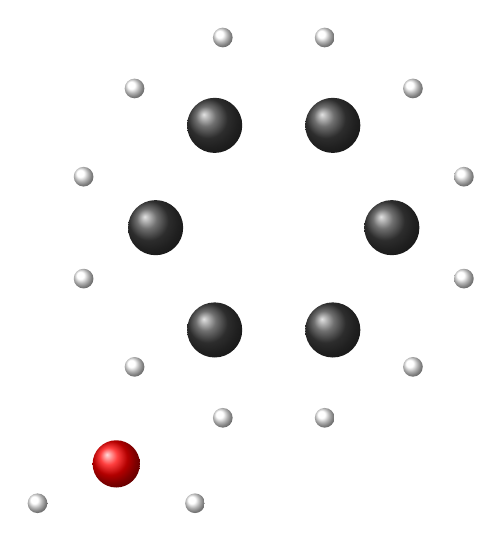
\begin{tikzpicture}
[   oxygen/.style={circle, ball color=red, minimum size=6mm, inner sep=0},
    hydrogen/.style={circle, ball color=white, minimum size=2.5mm, inner sep=0},
    carbon/.style={circle, ball color=black!75, minimum size=7mm, inner sep=0}
]
    \node[oxygen] (O1) at (0,0) {};
    \node[hydrogen] (H1) at (1,-0.5) {};
    \node[hydrogen] (H2) at (-1,-0.5) {};
    \SingleBond{O1}{H1}
    \SingleBond{O1}{H2}

    \foreach \c in {1,...,6}
    {   \node[carbon] (C-\c) at ($(2,3)+(\c*60:1.5)$) {};
        \node[hydrogen] (H-\c-a) at ($(2,3)+(\c*60-15:2.5)$) {};
        \node[hydrogen] (H-\c-b) at ($(2,3)+(\c*60+15:2.5)$) {};
        \RedBond{C-\c}{H-\c-a}
        \BlueBond{C-\c}{H-\c-b}
    }
    \foreach \c [evaluate={\c as \n using int(mod(\c,6)+1)}] in {1,...,6}
    {   \GreenBond{C-\c}{C-\n}
    }
\end{tikzpicture}

\end{document}
